\section{Performance Analysis}
	
	System implementation has been performed on a Atlys \texttrademark Spartan-6 Digilent platform \cite{atlys}, 
	cores used are the MicroBlaze v8.40 \cite{xilinx_microblaze} running an XilKernel v5.01a \cite{xilinx_xilkernel}
	operating system. Interconnected with Time Petri Processor by AXI bus\cite{xilinx_axi}.
	
	To verify the correct operation and analyze the IP Core synchronization times, measurements were 
	made for different numbers of iterations and number of threads trying to access a shared variable 
	in mutual exclusion. Then we compared the Petri Processor with an implementation using semaphores, 
	both solving the same problem. The choice of this second synchronization method is based on that 
	they are the lightest mechanism to perform these tasks.
	
	From these measurements, Speedup was calculated. The results are shown in Figure \ref{fig:speedup}, 
	where can be observed that for all cases, the processor is on average between 15\% and 30\% faster 
	than use of semaphores to solve the trouble of synchronizing multiple threads that want to accesses 
	a shared resource and even show peaks up to 70\%.
	
	These measurements were performed with times $\tau$ zero, in this way the performance is the same that i
	s obtained in the Petri Net Processor without temporal semantics. This is valid because the transition's
	time is part of the model, so, it is the same for the processor as for semaphore implementation.

		\begin{figure}[h]
			\centering
			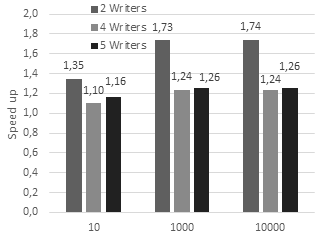
\includegraphics[width=0.85\linewidth]{./img/petri_speedup}
			\caption{Synchronization Speedup per iteration}
			\label{fig:speedup}
		\end{figure}
		
	As observed in Figure \ref{fig:simulation}, the processor needs only one half-clock cycle since the 
	counter reaches the value $\tau$ until a shot is placed in the output queue. The delay introduced is 
	insignificant in relation to the time takes a $\delta t$ of one clock cycle.
	
		\begin{figure}[h]
			\centering
			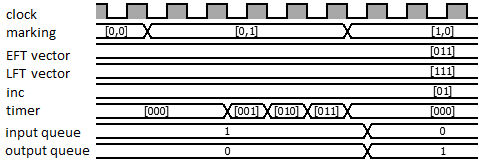
\includegraphics[width=0.95\linewidth]{./img/time}
			\caption{Running on hardware}
			\label{fig:simulation}
		\end{figure} 	
	
	Taking into account how insignificant the latency is and taking the time as part of the model it 
	is possible to analyze the performance without taking into account the vector $\Gamma$.	
	